\subsection{Downstream: does better labelling help the recommender?}\label{sec:nn-downstream}

A labeller is only worth what it changes. Three downstream tests follow, one simulated and two on real
data, and they do not all point the same way.

\paragraph{Simulation: the label-quality bottleneck closes.} Experiment E3
(Section~\ref{sec:ablations}) measured how much early weak-category targeting depends on label
quality, by drawing each observed label from the labeller's measured $P(\text{predicted} \mid
\text{true})$. Rerunning it with PuzzleNet's confusion matrix, on the same 200 seeds so that every
comparison is paired:

\begin{table}[H]
\centering
\small
\caption{Weak-category targeting over the first 30 puzzles, by the source of the game evidence
(200 paired runs, $T = 60$).}\label{tab:nn-labelsim}
\begin{tabularx}{\linewidth}{Xcc}
\toprule
\textbf{Label source} & \textbf{Beta-TS} & \textbf{IRT-TS} \\
\midrule
No game evidence              & 0.148 & 0.151 \\
Rule-based tagger             & 0.189 & 0.226 \\
\textbf{PuzzleNet}            & \textbf{0.245} & \textbf{0.306} \\
Perfect labels                & 0.239 & 0.321 \\
\bottomrule
\end{tabularx}
\end{table}

\begin{finding}[PuzzleNet labels are statistically indistinguishable from perfect ones]
For the IRT policy, PuzzleNet beats the rule-based tagger by $+0.080$ targeting
(95\% CI $+0.055$ to $+0.105$, $p = 7 \times 10^{-10}$, $d_z = 0.46$), and the remaining gap to
\emph{perfect} labels is $+0.015$ and not significant ($p = 0.31$). It closes 84\% of the
rules-to-perfect gap for IRT-TS and all of it for Beta-TS. Cumulative regret falls from 62.6 to 55.3,
against 53.2 with perfect labels. The bottleneck identified in E3 is, in simulation, gone.
\end{finding}

\begin{figure}[H]
\centering
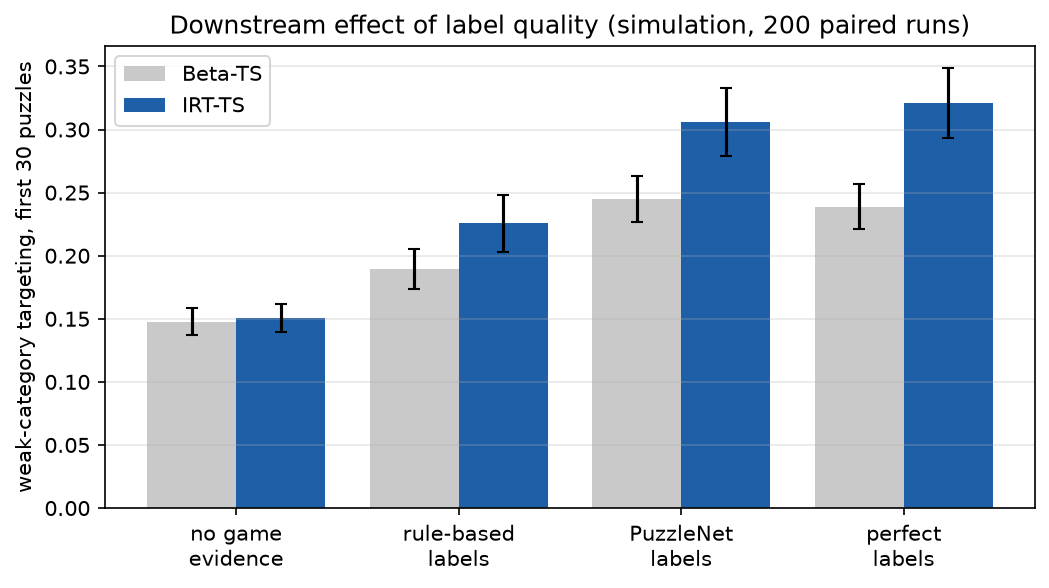
\includegraphics[width=0.8\linewidth]{figures/nn_label_simulation.png}
\caption{Downstream effect of label quality on early weak-category targeting (200 paired runs). PuzzleNet's labels are not statistically distinguishable from perfect ones.}\label{fig:nn-labelsim}
\end{figure}

\paragraph{Real players: the labels change, the diagnosis does not.} The 300-player cohort was
relabelled. Every one of the 40{,}067 critical positions was re-analysed with Stockfish at the
analyzer's own settings, and the resulting engine lines were labelled twice, once by each labeller, so
that the two versions of the cohort differ only in the labeller. Re-running the rule-based tagger on
the fresh engine lines reproduces its stored label 94.1\% of the time, which says the pipeline is
stable; the two labellers, however, agree with each other on only 37\% of real game positions. They
disagree about what players face:

\begin{table}[H]
\centering
\small
\caption{What the two labellers say the 40{,}067 critical positions of 300 real players
are.}\label{tab:nn-cohort-share}
\begin{tabularx}{\linewidth}{Xcc}
\toprule
\textbf{Category} & \textbf{Rule-based} & \textbf{PuzzleNet} \\
\midrule
Quiet Move        & 35\% & 12\% \\
General (no motif) & 11\% & 32\% \\
Endgame           & $<$1\% & 14\% \\
Fork              & 12\% & 5\% \\
Hanging Piece     & 9\% & 9\% \\
\bottomrule
\end{tabularx}
\end{table}

Given that the two labellers score $\kappa = 0.78$ and $0.49$ against an independent reference on
engine lines, the network's picture is the more credible: most critical positions in real games carry
no nameable motif, and a large share are endgame technique, while the rule-based tagger was calling a
third of everything a quiet move. That matters beyond this experiment, because the population category
norms shipped in the application (Section~\ref{sec:player-model}) were fitted on the rule-based
labels.

What does \emph{not} change is the conclusion of Section~\ref{sec:cohort-results}. With PuzzleNet
labels, split-half reliability of a player's per-category hit rates stays at zero (mean $|r| = 0.09$
across the categories with enough support, against $0.15$ before; the noise-corrected between-player
standard deviation is 0.0 under both labellings), and the ranking of the weakness models is unchanged.

\begin{finding}[Label noise was not the reason weaknesses looked like noise]
Tripling macro recall and nearly doubling $\kappa$ leaves per-category reliability at zero. The
earlier negative result therefore survives its most obvious challenge: it is not an artefact of a
crude labeller. From about 40 games, a player's per-category hit rates carry no stable
person-specific signal, whoever does the labelling, so personal weakness has to be learned online from
puzzle attempts rather than read off past games.
\end{finding}

\paragraph{Real logs: the difficulty estimate does not transfer to mined puzzles.} The third test is
the prequential replay of the application's own 123 attempts. Replacing the miner's formula with
PuzzleNet's difficulty makes the calibration \emph{worse}: log loss rises from 0.599 to 0.754.

The reason is visible in the numbers. For the 44 mined puzzles in the logs, PuzzleNet predicts a
difficulty 493 rating points higher on average than the formula (1611 against 1118), yet players solve
86.7\% of mined puzzles, against 80.0\% of Lichess pool puzzles. A mined puzzle is a position from the
player's \emph{own} game, which they have already seen at the board; it is easier for its owner than
its content suggests, and no model trained on Lichess ratings can know that. The formula's low ratings
were arbitrary, but they happened to sit closer to the truth for this population.

\begin{honest}[Honest status: the difficulty head is not used to serve mined puzzles]
The application records PuzzleNet's difficulty and uncertainty on every mined puzzle, but serves the
formula's rating unless \code{MINED\_RATING=puzzlenet} is set. Fitting the offset that would correct
the transfer needs data: a single scalar fitted on these 123 attempts runs to the edge of its range
(1181 points), which is fitting the 84.6\% base rate rather than the difficulty. The honest position
is that the difficulty head is well calibrated where it was validated --- Lichess puzzles, where its
intervals cover what they claim --- and unvalidated where the system would use it. The uncertainty it
reports is used: it is what a mined puzzle carries into the Bayesian update once the offset is known.
\end{honest}
